%
% Firewall
%
% Aleph Objects Firewall
%
% Copyright (C) 2014, 2015, 2016 Aleph Objects, Inc.
%
% This document is licensed under the Creative Commons Attribution 4.0
% International Public License (CC BY-SA 4.0) by Aleph Objects, Inc.
%

\section{Overview}
Aleph Objects has recently deployed pfSense firewalls, replacing OpenBSD.
Most servers and workstations run GNU/Linux, which uses iptables.


\section{iptables}
iptables is part of the Netfilter project and has been included by default in
the Linux kernel for many years.

\begin{figure}[h!]
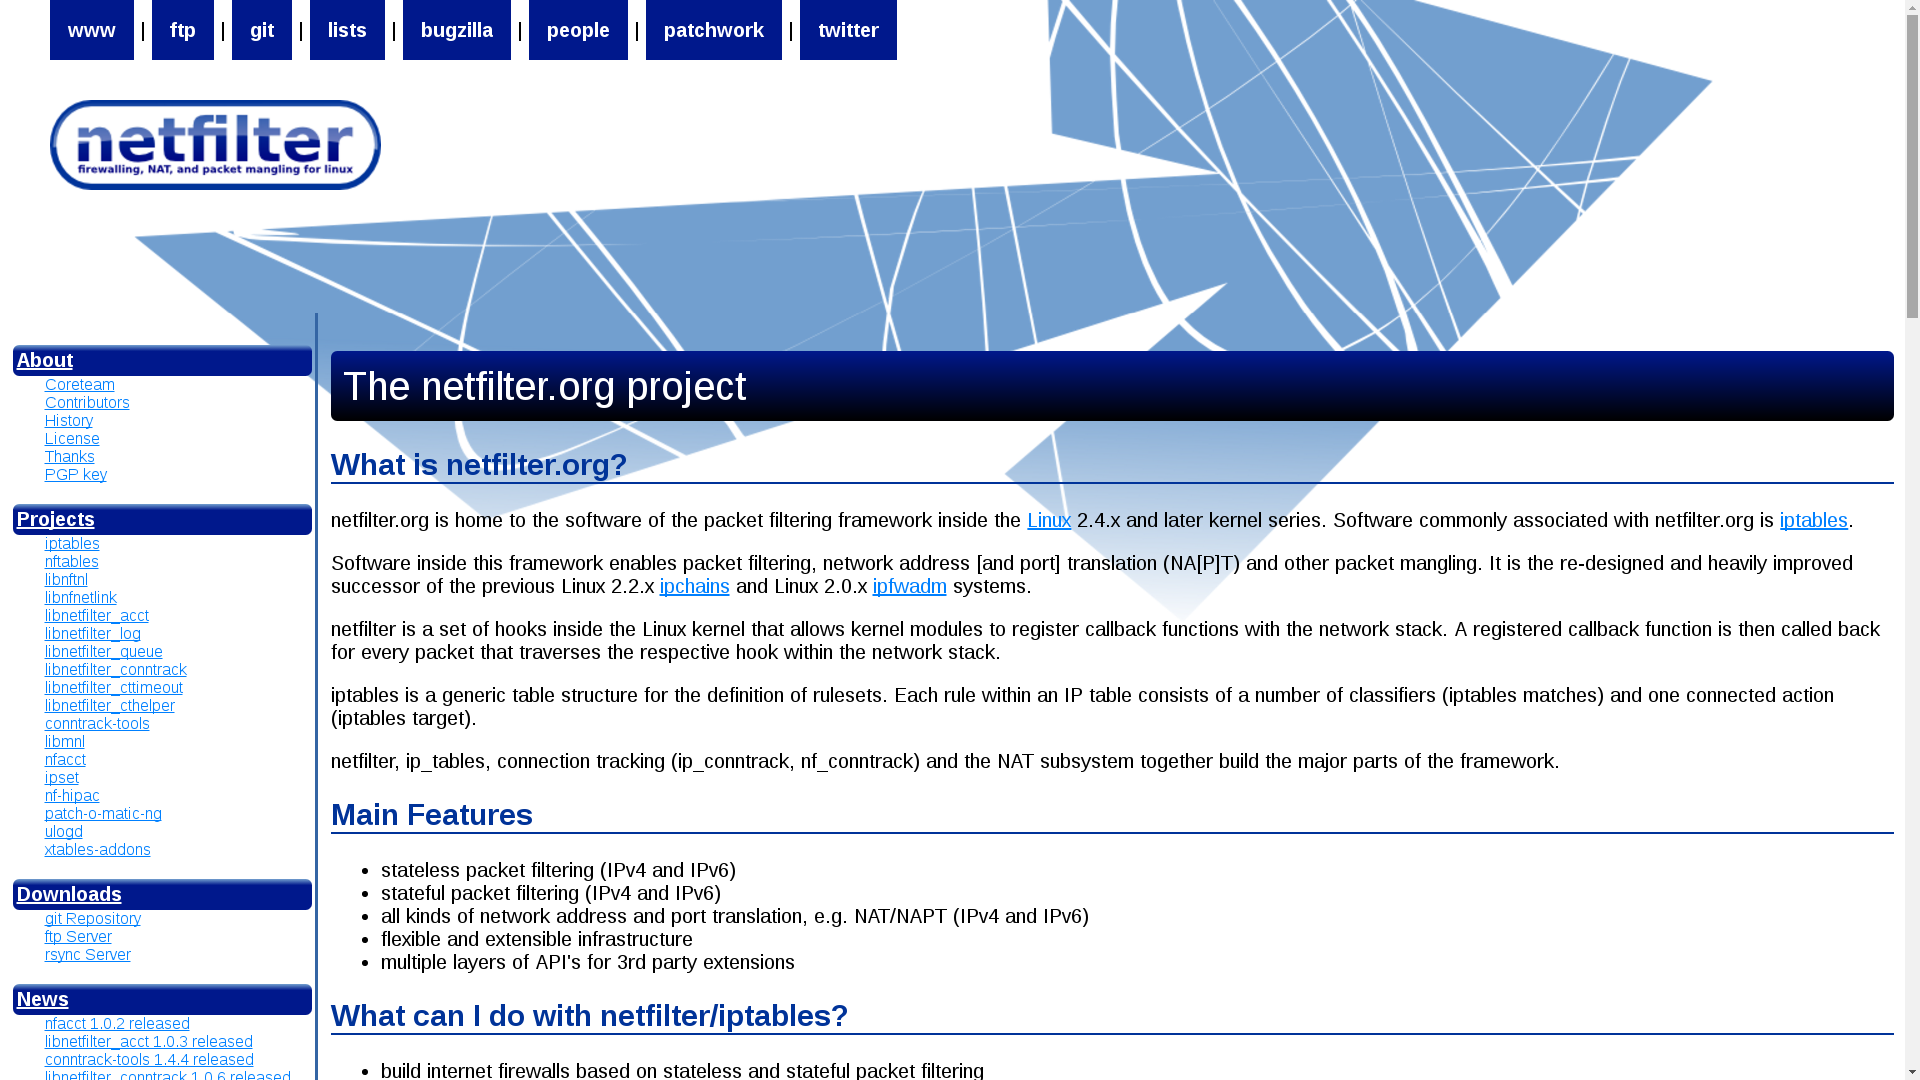
\includegraphics[keepaspectratio=true,height=1.10\textheight,width=1.00\textwidth,angle=0]{www-netfilter.png}
 \caption{Netfilter Website}
 \label{fig:www-netfilter}
\end{figure}

